% ====================================================================
% introduction.tex
% --------------------------------------------------------------------
% Introduction / functional description for the technical document
% template.
%
% Demonstrates:
%   - General descriptive text
%   - Mathematics with SI units (amsmath + siunitx)
%   - Cross-referencing (varioref + cleveref)
%   - Code listings from an external file
%   - Plots using pgfplots
%   - Timing Diagrams
%   - Citations
% ====================================================================

\section{Template Overview}
\label{sec:templateOverview}

\lettrine[lines=2, slope=0em, loversize=0.14, nindent=0pt, lhang=0.3, lraise=0]{T}{HIS} \LaTeX{} template is intended for clear, consistent technical documentation
across a wide range of disciplines — engineering reports, research write-ups,
specifications, educational material, and university dissertations among them.
It provides a structured framework for presenting figures, calculations, code,
and supporting explanation in a way that is easy to read and review, and comes
with a selection of commonly used \LaTeX{} packages pre-configured. The
examples below happen to use an electronics worked example, but nothing in the
framework is specific to any one field; swap the example content for your own.

% --------------------------------------------------
% Package examples
% --------------------------------------------------
\subsection{Package Examples}

% --------------------------------------------------
% Mathematics with SI units (amsmath + siunitx)
% --------------------------------------------------
\subsubsection{Mathematics with SI Units}

As an example, consider the emitter resistor from a simple bias network. With
an emitter voltage of \qty{1.65}{\volt} and an emitter resistor of
\qty{330}{\ohm}, the emitter current is

\begin{align}
  \label{eq:biasCurrent}
  I_{\text{E}}
    &= \frac{V_{\text{E}}}{R_{\text{E}}}
     = \frac{\qty{1.65}{\volt}}{\qty{330}{\ohm}}
     \approx \qty{5.0}{\milli\ampere}.
\end{align}

Using this current, the power dissipated in the resistor can be estimated as

\begin{align}
  P_{R_{\text{E}}}
    &= I_{\text{E}}^{2} R_{\text{E}}
     \approx \bigl(\qty{5.0}{\milli\ampere}\bigr)^{2}
              \cdot \qty{330}{\ohm}
     \approx \qty{8.3}{\milli\watt}.
\end{align}

Here, \texttt{siunitx} is used to keep all numerical values and units formatted
consistently via \verb|\qty{...}{...}| and \verb|\unit{...}|, while \texttt{mathtools}
and \texttt{amsmath} provide the aligned equations.

% --------------------------------------------------
% Code listings from external files
% --------------------------------------------------
\subsubsection{Code Listings}

Source code can be included directly from external files using the \texttt{listings} package (or \texttt{minted}, which is available as an optional extra). For example:

% ====================================================================
% codeExample.tex
% --------------------------------------------------------------------
% Example code using listing.
% ====================================================================

\begin{lstlisting}[caption={Code Example}, label={lst:codeExample}, language=C]
#include <stdio.h>

int main() {
   printf("Hello, World!"); /*printf() outputs the quoted string*/
   return 0;
}
\end{lstlisting}


% --------------------------------------------------
% Cross-referencing (varioref + cleveref)
% --------------------------------------------------
\subsubsection{Cross-Referencing}

The template uses \texttt{varioref} and \texttt{cleveref} to provide flexible
cross-references. Headings, equations, figures and tables can be labelled once
and then referred to consistently throughout the document.

For example, the general overview for this template is explained in
{\vref{sec:templateOverview}}. If that section moves to a different
page during editing, the reference text is updated automatically to reflect the
new location (for example, “section~1.2 on page~3” or “section~1.2 on the
previous page”).

% --------------------------------------------------
% pgfplots
% --------------------------------------------------
\subsubsection{Plots}

This figure shows a simple time-domain plot created directly in \LaTeX\ using the \verb|pgfplots| package.

% ====================================================================
% examplePlot.tex
% --------------------------------------------------------------------
% Example plot using pgfplots.
% ====================================================================

\begin{figure}[htbp]
\centering
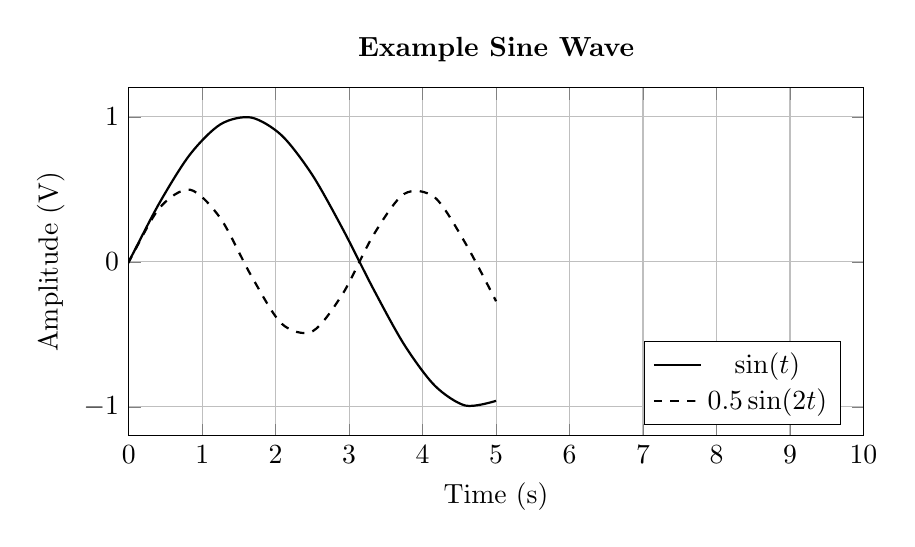
\begin{tikzpicture}
\begin{axis}[
  width=0.9\linewidth,
  height=6cm,
  grid=both,
  xmin=0, xmax=10,
  ymin=-1.2, ymax=1.2,
  xlabel={Time (s)},
  ylabel={Amplitude (V)},
  title={\textbf{Example Sine Wave}},
  legend pos=south east,
]
\addplot[smooth, thick] {sin(deg(x))};
\addlegendentry{$\sin(t)$}

\addplot[smooth, thick, dashed] {0.5*sin(deg(2*x))};
\addlegendentry{$0.5\sin(2t)$}
\end{axis}
\end{tikzpicture}
\caption{Example plot generated directly in \LaTeX\ using \texttt{pgfplots}.}
\label{fig:example-plot}
\end{figure}

% --------------------------------------------------
% timing diagrams
% --------------------------------------------------

\subsubsection{Timing Diagrams}

\Vref{fig:timing-example} shows an example digital timing diagram created directly in \LaTeX\ using the \texttt{tikz-timing} package. The diagram includes a free-running clock, an active-low reset pulse, a data signal, and a \texttt{VALID} strobe indicating when the data should be sampled.

% ====================================================================
% exampleTiming.tex
% --------------------------------------------------------------------
% Example timing diagram using tikz-timing.
% ====================================================================

\begin{figure}[H]
\centering
\begin{tikztimingtable}[
  timing/slope=0,
  timing/xunit=10mm,   % <-- horizontal scale (pick what looks right)
  timing/yunit=7.5mm    % <-- vertical scale
]
  CLK   & 8{C} \\
  nRST  & 2H 2L 4H \\
  DATA  & 2L 2H 2L 2H \\
  VALID & 4L 2H 2L \\
\end{tikztimingtable}
\caption{Example timing diagram generated with \texttt{tikz-timing}.}
\label{fig:timing-example}
\end{figure}

% --------------------------------------------------
% Bibliography Reference
% --------------------------------------------------
\subsubsection{Citations and Bibliography}

The optical transmission of ceramics can be estimated using simplified scattering models; this is described in “A new closed-form expression is presented for estimating the real-in-line transmission of ceramics consisting of non-absorbing phases in dependence of the inclusion or pore size” \cite{pabst_mie_approx_2013}. This section demonstrates how to cite a source, in IEEE format, in text and automatically generate a bibliography.



